\newpage
\begin{section}{Algebra}

\begin{subsection}{factorization}
\begin{enumerate}
	\item common factor
	\item common factor by agroupation of terms
	\item cubic differences
	\item perfect square trinomial
	\item trinomial of the form $x^2 + bx + c $ 
	\item trinomial of the form $ax^2 + bx + c $
	\item sum and difference of cubes
	\item sintetic divition
	\item general formula
\end{enumerate}
\end{subsection}

\newpage
	\begin{subsection}{Sintetic divition}
		Example:
		$$x^3 - 5x^2 + 2x + 8$$
		Taking the divisors of the independent term
		$$p = D_8 = \{\pm 1, \pm 2, \pm 4, \pm 8 \} $$
		and the divisors of the term with the highest exponent
		$$q = D_1 = \{\pm 1\} $$
		$$p/q = \{\pm 1, \pm 2, \pm 4, \pm 8 \} $$
		now all the posibilities are in the space p/q that are integers

		so:
		\begin{center}
		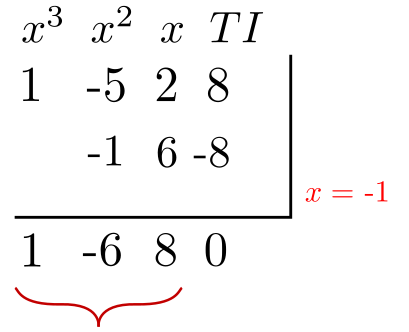
\includegraphics[scale = 0.8]{1.png}
		\end{center}
		then:

		$$(x^2 - 6x +8)(x+1) $$
		then:
		$$(x+1)(x-4)(x-2)$$
	\end{subsection}

	\begin{subsection}{cubic differences}
	$$u^3 + 1 = (u^2-u+1)(u+1)$$
	$$u^3 - 1 = (u^2+u+1)(u-1)$$
	\end{subsection}

	\begin{subsection}{general formula}
		$$x= \frac{ -b \pm \sqrt{b^2 - 4ac}}{2a}$$
	\end{subsection}


\end{section}
